% !TEX root = ../../numb3rs.tex
\newpage
\subsection{303: Provenance\label{303}}

In this episode a famous paint is stolen and the FBI team is involved in the case. The case complicates quickly, as they discover that the Nazis looted the house of the original paint's owner. Charlie uses mathematical models and discovers that the paint stolen was a fake. To complicate matters, there is a murder plot involved. \\

%%%%%%%%%%
\temph{Network Diffusion}
%%%%%%%%%%

Several models have been used to understand network diffusion. The word diffusion simply means ``movement of the object''. The problem here is to understand what makes objects move through a network (a graph) For instance, what makes rumors, diseases spread? In this episode is used to find out the possible location of a stolen pain. \\

\fbox{\begin{minipage}{43em}
\begin{center} \large \dotuline{Tangent}  \\ \end{center}
Network diffusion is a very active field nowadays, partially because of the popularity of social networks on the internet such as Facebook or MySpace. There are many questions that arise in this field: how do people make friends? How likely is that you will join a group or post a message if your friends have already done so. Mathematical models of several kinds are used to understand the behavior of these networks, such as the construction of \bref{random graphs}{https://en.wikipedia.org/wiki/Random_graph} with given constraints. Below we have a partial subgraph from Facebook, where people are vertices and are connected to other people if they are friends as defined by Facebook. 
	\begin{figure}[H]
	   \centering
	   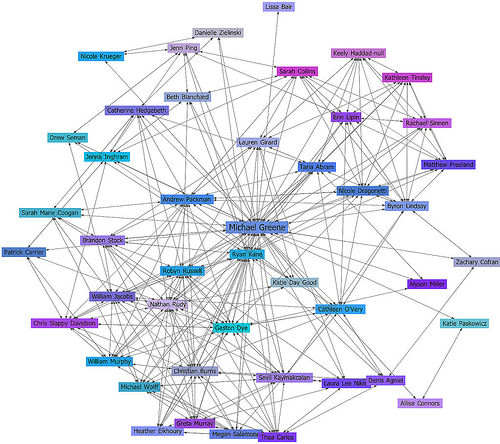
\includegraphics[width=0.5\textwidth]{season3/303/images/social_net.jpg} 
	\end{figure}
\end{minipage}} \vspace{0.2cm}


\noindent\textbf{\large Network diffusion probability models} \\

At some point, Charlie is trying to find out the possible places where the stolen paint can be sold. In order to do this, he uses a \emph{network diffusion probability model}. Let us focus on the details of these models. First of all, the network is represented by a directed, weighted graph, where the weights represent the probability of diffusion. For instance, consider the graph below 
	\begin{figure}[H]
	   \centering
	   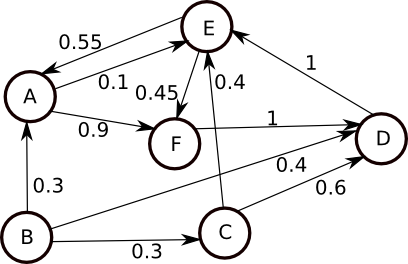
\includegraphics[width=0.35\textwidth]{season3/303/images/net_dif.png} 
	\end{figure}

Notice that from point there are two places to move from point A; that is, F and E. An object located at A moves to F with a probability of 0.1, whereas the same object moves to F with probability 0.9. Notice that the sum of all the weights of edges going \emph{out} of any point is 1. \\

One can encode the a weighted graph in an \emph{adjacency matrix}, which consists of a rectangular array, where entry $(i,j)$ is the weight of the edge from $i$ to $j$. For instance, the above graph is encoded as follows:
	\[
	\begin{pmatrix}
	0 & 0 & 0 & 0 & 0.1 & 0.9 \\
	0.3 & 0.3 & 0.4 & 0 & 0.1 & 0.9 \\
	0 & 0 & 0 & 0.4 & 0.6 & 0 \\ 
	0 & 0 & 0 & 0 & 1 & 0 \\
	0.55 & 0 & 0 & 0 & 0 & 0.45 \\
	0 & 0 & 0 & 1 & 0 & 0 \\ 
	\end{pmatrix}
	\]


\fbox{\begin{minipage}{43em}
\begin{center} \large \dotuline{Activity 1}  \\ \end{center}
\begin{enumerate}[i.]
\item Let $M$ be the above matrix, and $N=[1, 0, 0, 0, 0, 0,]$ be the matrix representing point $A$. What does $N\times M$ represent? What about $N\times M^2$ and $N\times M^k$ for a positive integer $k$?
\item Use a calculator or a computer and find the value of $N\times M^k$ for several $k$ up to 4 digits. Do you notice anything unusual?
\item In the previous problem, at some point the product $N\times M^k = N\times M^{k+1}$. In this case, we say that the product stabilizes
\item Consider the following statement: ``For any matrix M, there exists a positive $k$ so that the product $N\times M^k$ stabilizes''. Is this statement true? If so try to argue why. Otherwise provide a counterexample.
\end{enumerate}
\end{minipage}} \vspace{0.2cm}

%%%%%%%%%%
\temph{Network Diffusion}
%%%%%%%%%%

There are many applications where one is interested in network diffusion; for instance, the spread of diseases, evolution of species, spread of rumors, population dynamics, etc. We present a very simple model of the population dynamics, called the \emph{Moran process}. The process is the following: A population is represented in a weighted graph, at each step one chooses a vertex $v$ to reproduce, and pick one of its neighbors $u$ to replace it with a copy of $v$. The picture below is represents this model: We pick the red vertex to reproduce, a neighbor to be replaced (the one connected with the red edge) and replace the blue vertex with a copy of the red one. In the picture below we have not included the weights, for simplicity. The model also puts weight on the vertices, representing the \emph{fitness} of red or blue vertices 
	\begin{figure}[H]
	  \centering
	  \begin{minipage}[b]{0.2\textwidth}
	    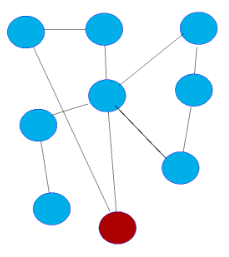
\includegraphics[width=\textwidth]{season3/303/images/dots1.png}
	  \end{minipage}
	  \hspace{3cm}
	  \begin{minipage}[b]{0.2\textwidth}
	    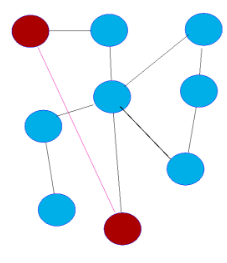
\includegraphics[width=\textwidth]{season3/303/images/dots2.png}
	  \end{minipage}
	\end{figure}

\fbox{\begin{minipage}{43em}
\begin{center} \large \dotuline{Activity 2}  \\ \end{center}
\begin{enumerate}[i.]
\item We say that a Moran process reaches \emph{fixation} if there is a step in the process where all the vertices are either red or blue (since at this point, any step will not change the color of any vertex). Give an example of a process that starts with all blue vertices, then a red vertex is introduces, and at some point all the vertices will become red. Give another example where the red vertices will eventually disappear.
\item For a graph $G$ with all its vertices blue, define $M_G$ to be the minimal number of red vertices that need to be introduced (that is, the minimum number of blue vertices that need to be turned red) in order to guarantee a red fixation. Give examples of two graphs on n vertices (for any n) such that $M_G = 1$, and $M_G = n - 1$. Notice that $M_G$ does not depend on the weights of the edges.
\item Let us look at the Moran process of the graph G be the directed 4-cycle $A \rightarrow B \rightarrow C \rightarrow D \rightarrow A$ (where $A$, $B$, $C$, and $D$ are the vertices). Suppose that there are 3 blue vertices and one red vertex, and that the fitness of the red vertex is 10, while the fitness of the blue vertices is 1. If we select vertices with probability proportional to their fitness, what is the probability of choosing a red vertex for reproduction at the first step of the process? What about the probability of selecting a blue vertex?
\item With the sam considerations as above, consider the Moran process at its fifth step. What is the probability of reaching red fixation at the fifths step? What about blue fixation?
\end{enumerate}
\end{minipage}} \vspace{0.2cm}

